\documentclass[11pt,a4paper]{article}

% --- Paquetes de configuración básica y tipografía ---
\usepackage[utf8]{inputenc}
\usepackage[spanish,es-tabla]{babel}
\usepackage[margin=2.5cm]{geometry}
\usepackage{amsmath,amsfonts,amssymb}
\usepackage{graphicx}
\usepackage{booktabs}
\usepackage{tabularx}
\usepackage{longtable}
\usepackage{array}
\usepackage{caption}
\usepackage{subcaption}
\usepackage{float}
\usepackage{xcolor}
\usepackage{listings}
\usepackage{fancyhdr}
\usepackage{microtype}
\usepackage{enumitem}
\usepackage[hidelinks,colorlinks=true,linkcolor=blue!70!black,citecolor=blue!70!black,urlcolor=blue!70!black]{hyperref}

% --- Configuración de encabezados y pies de página ---
\pagestyle{fancy}
\fancyhf{}
\rhead{\footnotesize CC209 -- Data Mining Tools | TF1}
\lhead{\footnotesize Estimación y Tasación Inmobiliaria en Lima Metropolitana}
\cfoot{\thepage}

\title{\vspace{-1.5cm}\textbf{Universidad Peruana de Ciencias Aplicadas (UPC)}\\
\large Facultad de Ingeniería -- Carrera de Ciencias de la Computación\\
\vspace{0.3cm}
\Large \textbf{CC209: Data Mining Tools -- Trabajo Final (TF1)}\\
\vspace{0.4cm}
\LARGE \textbf{Sistema Inteligente de Tasación y Estimación de Precios de Departamentos en Lima Metropolitana: Enfoque de Ensamble Ponderado sobre Valor Unitario ($\text{US\$/m}^2$) con Explicabilidad SHAP}}
\author{\textbf{Equipo de Proyecto Integrador}\\
Docente: Carlos Fernando Montoya Cubas}
\date{Ciclo 2026-1}

\begin{document}

\maketitle

\begin{abstract}
El presente informe documenta la versión integrada, refinada y desplegada del Trabajo Final (TF1) para la estimación de precios de oferta de departamentos residenciales en Lima Metropolitana, a partir de la base de datos abiertos del Banco Central de Reserva del Perú (BCRP, 1998--2026). Frente al primer avance (TP1), se introducen cuatro mejoras metodológicas y técnicas sustantivas: (i) la transición del modelado de precios totales hacia la estimación del valor unitario por metro cuadrado ($\text{precio\_m2} = \text{precio\_usd} / \text{superficie\_m2}$) con reconstrucción en dólares, estabilizando la varianza residual en propiedades disímiles; (ii) la incorporación de una técnica no supervisada de la segunda mitad del curso consistente en un \textit{Clustering Espacial de Submercados} ($K$-Means, $k=4$) e ingeniería de tipologías de habitabilidad sin fuga de datos; (iii) una optimización bayesiana sistemática con Optuna sobre un esquema de validación temporal triple out-of-time (2022--2026), culminando en un Ensamble Heterogéneo Calibrado de 5 modelos (CatBoost 28.1\%, Random Forest 21.7\%, LightGBM 22.1\%, XGBoost 27.4\%, Ridge 0.7\%); y (iv) un módulo profundo de interpretabilidad basada en teoría de juegos (TreeSHAP) y diagnóstico de colas de error. Evaluado sobre una partición de prueba ciega temporal de dos años (2024--2026, $N=25,042$), el ensamble final alcanza un Error Porcentual Mediano (\text{MedAPE}) de \textbf{11.11\%}, un MAE de \textbf{\$22,650} y un RMSE de \textbf{\$32,063}, superando con holgura a la regla empírica del mercado inmobiliario (MedAPE 14.90\%) y clasificando con éxito al \textbf{45.77\%} de los inmuebles dentro del margen estricto del $\pm 10\%$ de error. La solución se materializa en una aplicación interactiva en Streamlit conectada al pipeline serializado para cotizaciones en tiempo real.
\end{abstract}

\vspace{0.3cm}

\section{Evolución Metodológica Respecto al TP1}

El Trabajo Final no constituye una simple extensión cosmética del TP1, sino una evolución fundamentada en la evidencia empírica obtenida tras el diagnóstico del primer avance. La Tabla~\ref{tab:evolucion_tp1_tf1} sintetiza los cambios obligatorios introducidos, sus motivaciones técnicas y su impacto comprobado.

\begin{table}[H]
\centering
\small
\caption{Matriz de Evolución Técnica: Trabajo Parcial (TP1) frente a Trabajo Final (TF1).}
\label{tab:evolucion_tp1_tf1}
\begin{tabularx}{\textwidth}{l p{3.2cm} p{4.2cm} X}
\toprule
\textbf{Elemento} & \textbf{Estado TP1} & \textbf{Evolución TF1} & \textbf{Motivo Técnico / Evidencia} \\
\midrule
\textbf{Variable Objetivo} & Predicción directa de $\text{precio\_usd}$ en $\log(1+y)$. & \textbf{Predicción de $\text{US\$/m}^2$} y reescalado: $\hat{y}_{\text{usd}} = \hat{y}_{\text{m2}} \cdot \text{m}^2$. & Desacopla el efecto de escala del tamaño, reduce la heterocedasticidad y disminuye el MAE en \$281 y RMSE en \$501. \\
\addlinespace
\textbf{Técnica Adicional} & \textit{Ninguna} (no requerida en semana 7). & \textbf{Clustering Espacial de Submercados} ($K$-Means, $k=4$). & Segmentación de distritos en macro-zonas homogéneas (Top, Moderna, Centro, Periferia) de acuerdo a la teoría inmobiliaria. \\
\addlinespace
\textbf{Variables e Ingeniería} & 6 atributos físicos crudos y distrito administrativo. & Ratios de habitabilidad (baños/hab, m²/hab, sup. relativa distrital) y tipología. & Caracteriza el confort y la amplitud interna, controlando la tipología del producto (monoambiente vs. penthouse). \\
\addlinespace
\textbf{Validación y Partición} & Split simple: Train 2022--2023 / Test 2024--2026. & \textbf{Partición Triple Out-of-Time}: Selección (Train/Val) y Test ciego final. & Garantiza cero data leakage en la selección de hiperparámetros y calibración de pesos. \\
\addlinespace
\textbf{Modelamiento} & Modelos individuales con hiperparámetros por defecto. & \textbf{Ensamble Heterogéneo Calibrado con Optuna} (CatBoost + RF + LightGBM + XGBoost + Ridge). & Reduce la varianza de estimación combinando múltiples arquitecturas no lineales (árboles simétricos, leaf-wise y Hessian) junto con regularización $L_2$. \\
\addlinespace
\textbf{Interpretabilidad} & Gráficos residuales y correlación básica. & \textbf{TreeSHAP Global y Local} (Beeswarm, Barras y Waterfall plots). & Permite auditar en dólares o unitario cuánto valor aporta cada atributo por inmueble cotizado. \\
\addlinespace
\textbf{Despliegue} & Exclusivamente en Jupyter Notebooks. & \textbf{Aplicación Web Interactiva en Streamlit} (\texttt{app.py}). & Cumple con el criterio de demostración funcional en tiempo real para la exposición de 12 minutos. \\
\bottomrule
\end{tabularx}
\end{table}

\section{Definición del Problema, Datos y Calidad}

\subsection{Delimitación del Problema}
La fijación del precio de oferta en Lima Metropolitana se realiza comúnmente mediante comparación heurística de anuncios contemporáneos del mismo distrito. Sin embargo, la heterogeneidad constructiva, los diferenciales de metraje y la dispersión entre zonas periféricas y consolidadas limitan la precisión de las reglas convencionales. El objetivo del proyecto consiste en predecir el **precio de oferta en dólares americanos** ($\text{precio\_usd}$) a partir del vector de atributos físicos y espaciales del inmueble, proporcionando al tasador un valor central y un intervalo empírico de negociación comercial ($\pm 11.1\%$).

\subsection{Procedencia y Base Depurada}
Los datos provienen de la Base Desagregada de Precios de Venta de Departamentos del Banco Central de Reserva del Perú (BCRP), compuesta originalmente por 119,980 anuncios trimestrales (1998--2026). Para el modelado contemporáneo se delimitó el estudio al período 2022-T1 a 2026-T1 (40,347 registros válidos en 22 distritos).
\begin{itemize}[leftmargin=*]
    \item \textbf{Limpieza Auditada:} Retiro estricto de 1,155 duplicados exactos y 17 exclusiones manuales de precios anómalos documentadas con hash criptográfico en \texttt{reports/auditoria\_preparacion/decisiones\_precios.csv}.
    \item \textbf{Aislamiento Anti-Leakage:} Exclusión obligatoria de variables derivadas del precio en moneda nacional (\texttt{precio\_soles}, \texttt{precio\_soles\_2009}) e indicadores macroeconómicos contemporáneos (\texttt{tipo\_cambio}, \texttt{ipc}).
\end{itemize}

\section{Flujo Metodológico e Ingeniería de Características}

\subsection{Selección y Justificación Sistemática del Número de Clusters ($K$)}
En el modelado no supervisado, fijar el número de clusters $k$ de manera arbitraria o puramente intuitiva constituye una debilidad metodológica severa. Para garantizar fundamentación empírica y justificar por qué $k=4$ es la partición idónea, se evaluó sistemáticamente el espacio de particiones sobre el conjunto de entrenamiento para $k \in [2, 7]$ mediante dos criterios rectores:
\begin{enumerate}
    \item \textbf{Método del Codo (Inercia intra-cluster / WCSS):} La reducción marginal de la inercia experimenta un punto de inflexión marcado en $k=4$ (caída de 19.12 a 13.48, reduciendo drásticamente la ganancia de varianza adicional para $k \ge 5$).
    \item \textbf{Coeficiente de Silueta (\textit{Silhouette Score}):} Para particiones con relevancia operativa ($k \ge 3$), $k=4$ alcanza el pico máximo de cohesión interna y separación con \textbf{0.4765}, superando sensiblemente a $k=3$ (0.4191) y $k=6$ (0.4167).
\end{enumerate}

\begin{figure}[H]
\centering
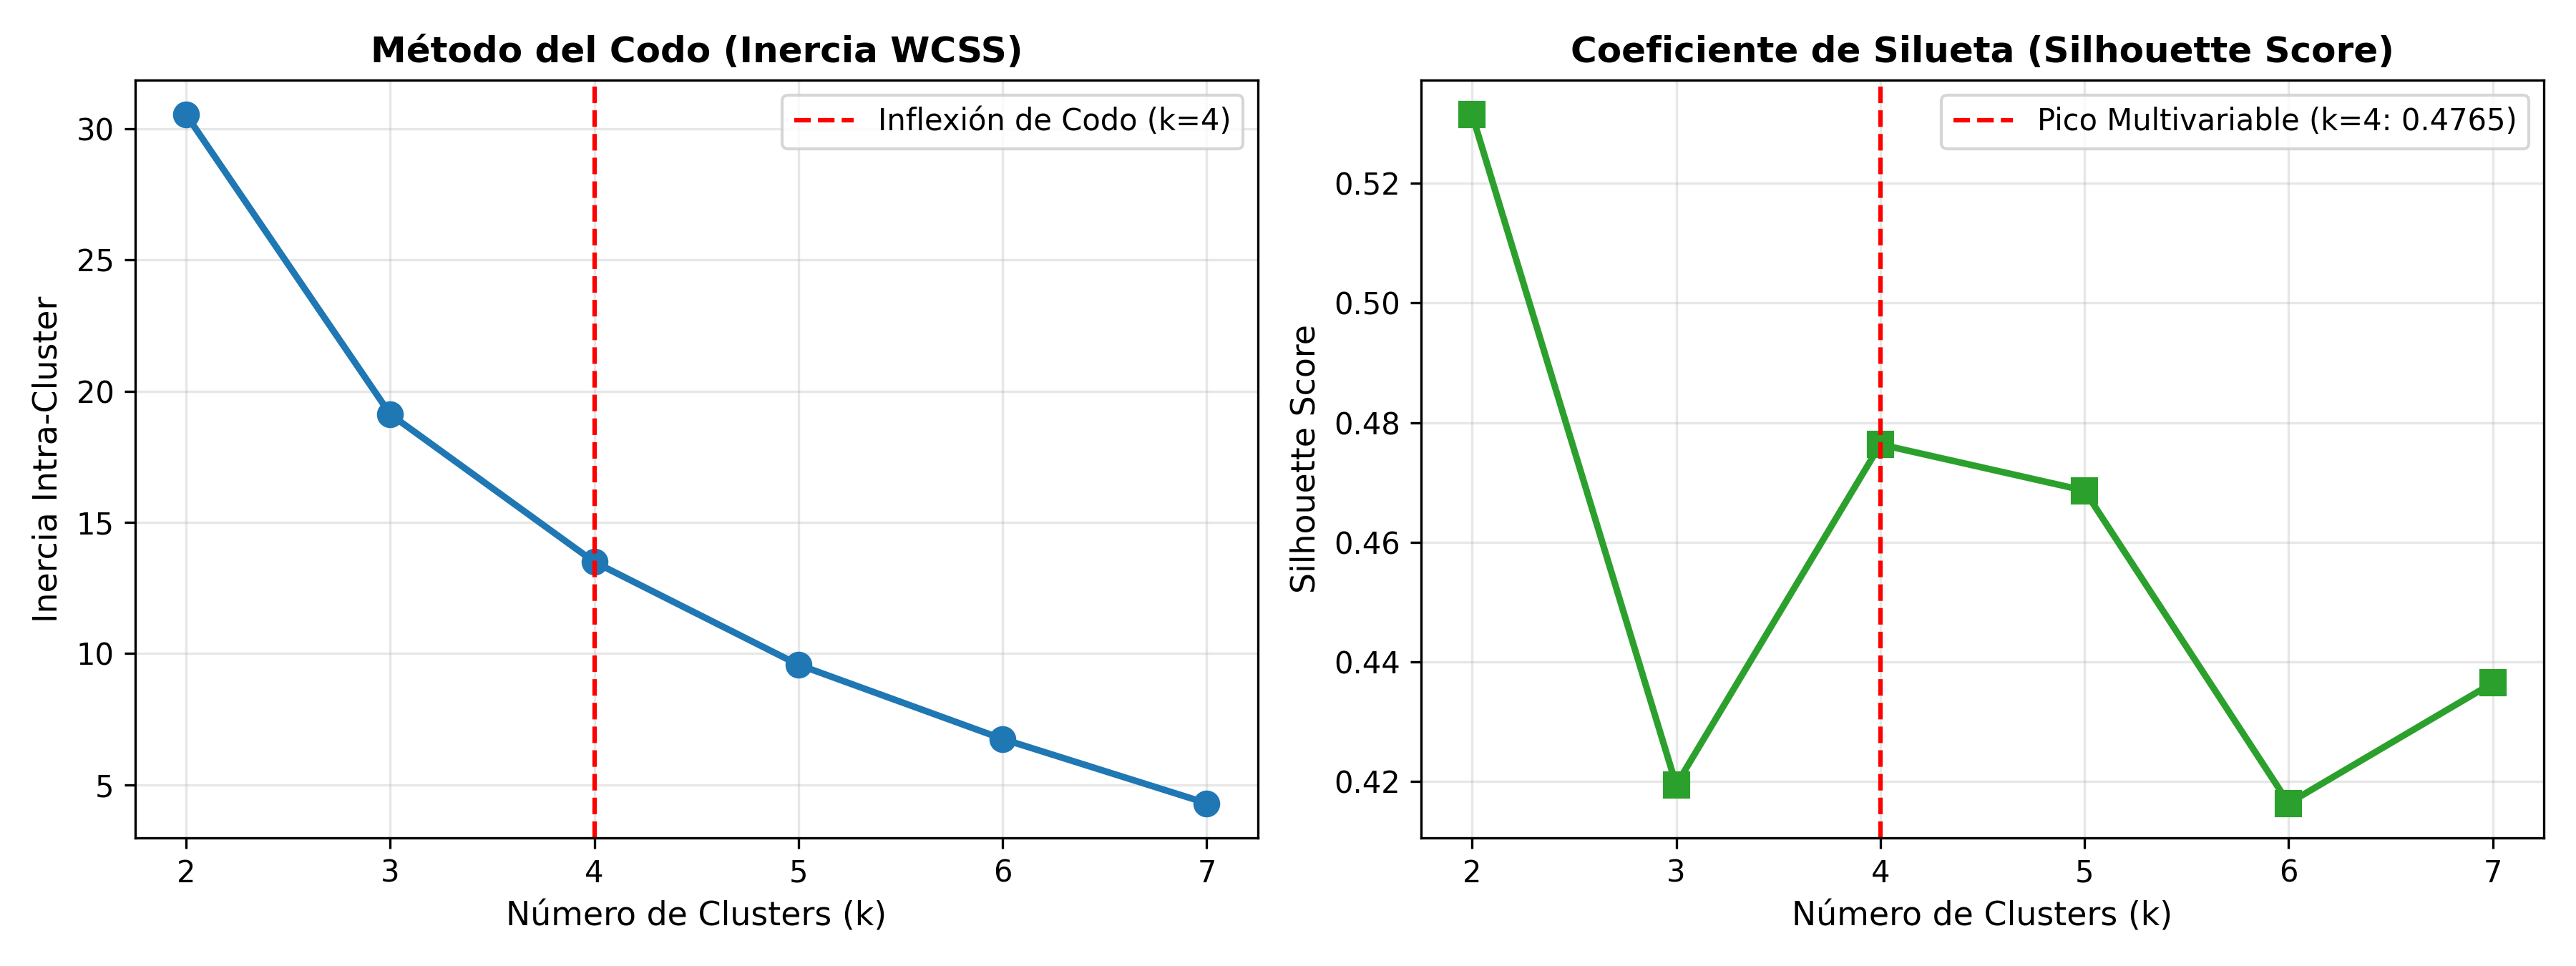
\includegraphics[width=0.88\textwidth]{reports/figures/04_seleccion_optima_k_clustering.png}
\caption{Evaluación sistemática de agrupamiento: Método del Codo (Inercia WCSS) y Coeficiente de Silueta para $k \in [2, 7]$. El codo y el pico multivariable confirman a $k=4$ como la partición óptima.}
\label{fig:seleccion_k}
\end{figure}

Bajo esta partición óptima validada ($k=4$), los 22 distritos de Lima Metropolitana quedan categorizados en cuatro macro-submercados socio-inmobiliarios homogéneos, cuyos perfiles enriquecidos se resumen en la Tabla~\ref{tab:perfiles_submercados}:

\begin{table}[H]
\centering
\small
\caption{Perfiles Enriquecidos de los 4 Macro-Submercados Inmobiliarios Descubiertos por $K$-Means.}
\label{tab:perfiles_submercados}
\begin{tabularx}{\textwidth}{l c c c c c c c X}
\toprule
\textbf{Submercado} & \textbf{\#Dist.} & \textbf{\%Mkt} & \textbf{Precio USD} & \textbf{US\$/m²} & \textbf{m²} & \textbf{Antig.} & \textbf{Gar.} & \textbf{Distritos Integrantes} \\
\midrule
\textbf{Lima Top} & 5 & 35.4\% & \$195,000 & \$1,927 & 103 m² & 11 a. & 1.0 & La Molina, Miraflores, San Borja, San Isidro, Surco \\
\addlinespace
\textbf{Lima Moderna} & 7 & 40.6\% & \$130,000 & \$1,685 & 79 m² & 7 a. & 1.0 & Barranco, Jesús María, Lince, Magdalena, Pueblo Libre, San Miguel, Surquillo \\
\addlinespace
\textbf{Lima Centro / Tradicional} & 8 & 21.2\% & \$89,000 & \$1,150 & 75 m² & 8 a. & 0.0 & Ate, Bellavista, Breña, Cercado, Chorrillos, La Perla, La Victoria, Los Olivos \\
\addlinespace
\textbf{Lima Periferia Norte} & 2 & 2.8\% & \$55,000 & \$727 & 74 m² & 5 a. & 0.0 & Carabayllo, Comas \\
\bottomrule
\end{tabularx}
\end{table}

\begin{figure}[H]
\centering
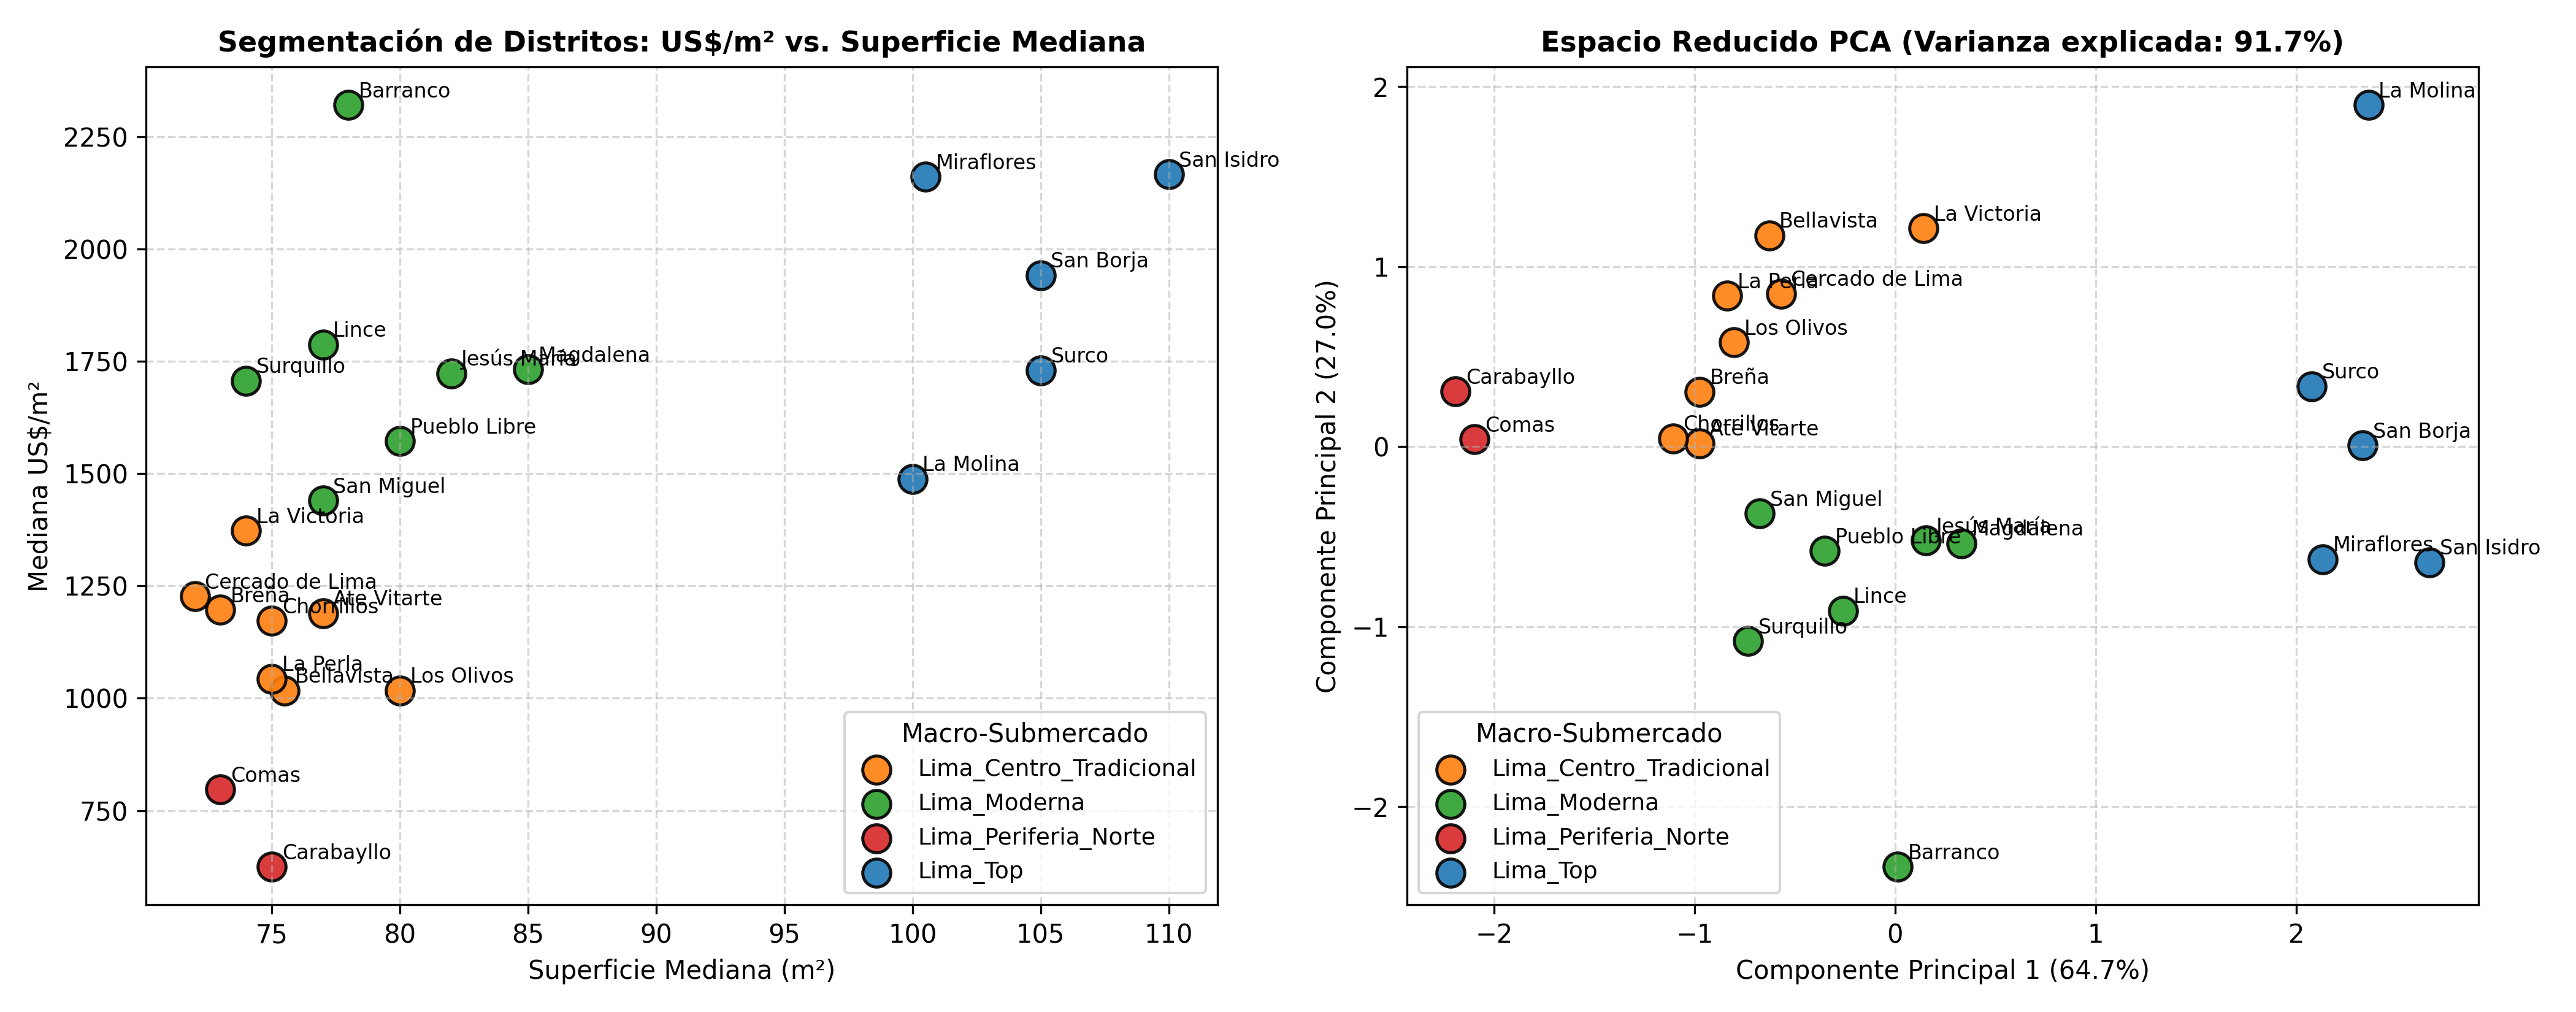
\includegraphics[width=0.95\textwidth]{reports/figures/05_visualizacion_clusters_submercados.png}
\caption{Visualización espacial de los 4 Macro-Submercados Inmobiliarios identificados por $K$-Means. Izquierda: Dispersión distrital en el plano físico (Mediana US\$/m² vs. Mediana Superficie). Derecha: Proyección en Componentes Principales (PCA) capturando la separación multivariada de los submercados.}
\label{fig:visualizacion_clusters}
\end{figure}

\subsection{Ingeniería de Ratios de Habitabilidad}
Se generaron variables funcionales que capturan el confort sin generar data leakage:
\begin{equation}
\text{ratio\_banos\_habitacion} = \frac{\text{baños}}{\max(\text{habitaciones}, 1)}, \quad \text{m2\_por\_habitacion} = \frac{\text{superficie\_m2}}{\max(\text{habitaciones}, 1)}
\end{equation}
\begin{equation}
\text{ratio\_sup\_distrital} = \frac{\text{superficie\_m2}}{\text{Mediana}(\text{superficie})_{\text{distrito}}^{\text{Train}}}
\end{equation}
Adicionalmente, se segmentó la variable categórica \texttt{tipologia} (\textit{Estudio Compacto}, \textit{Familiar Estándar}, \textit{Familiar Amplio}, \textit{Premium Penthouse}).

\section{Experimentación Sistemática y Ensamble Ponderado}

\subsection{Estrategia de Validación Cronológica Out-of-Time}
Para impedir que la selección de hiperparámetros contamine la evaluación final, se articuló una partición temporal triple:
\begin{enumerate}
    \item \textbf{Entrenamiento de Selección (2022-T1 a 2023-T2, $N=10,048$):} Ajuste de centroides, imputadores, escaladores y estimadores preliminares.
    \item \textbf{Validación de Selección (2023-T3 a 2023-T4, $N=5,101$):} Optimización bayesiana con Optuna para hiperparámetros de árboles y ponderación del ensamble.
    \item \textbf{Reentrenamiento Final (2022-T1 a 2023-T4, $N=15,156$):} Ajuste del pipeline sobre toda la historia previa disponible.
    \item \textbf{Prueba Ciega Out-of-Time (2024-T1 a 2026-T1, $N=25,042$):} Evaluación imparcial no vista durante ninguna etapa de modelado.
\end{enumerate}

\subsection{Calibración del Ensamble con Optuna}
Se entrenó un benchmark de cinco algoritmos heterogéneos ajustados sobre $\log(1 + \text{US\$/m}^2)$:
\begin{itemize}
    \item \textbf{CatBoost Regressor:} Árboles simétricos (*oblivious trees*) optimizados con Optuna (\texttt{iterations=400}, \texttt{depth=7}, \texttt{lr=0.101}, \texttt{l2=6.22}).
    \item \textbf{LightGBM Regressor:} Crecimiento por hojas (*leaf-wise*) con control de profundidad (\texttt{n\_estimators=400}, \texttt{num\_leaves=63}, \texttt{lr=0.08}).
    \item \textbf{XGBoost Regressor:} Potenciación con regularización cuadrática Hessian (\texttt{n\_estimators=400}, \texttt{max\_depth=7}, \texttt{lr=0.08}, \texttt{reg\_lambda=6.0}).
    \item \textbf{Random Forest Regressor:} Embolsado de 100 árboles con profundidad máxima 16.
    \item \textbf{Ridge Regressor:} Regularización lineal $L_2$ con $\alpha=1.5$.
\end{itemize}
Los pesos del ensamble se optimizaron en validación mediante 150 trials de Optuna minimizando el MedAPE:
\begin{equation}
\hat{y}_{\log(\text{US\$/m}^2)} = 0.2815 \cdot \hat{y}_{\text{CB}} + 0.2166 \cdot \hat{y}_{\text{RF}} + 0.0068 \cdot \hat{y}_{\text{RD}} + 0.2209 \cdot \hat{y}_{\text{LGB}} + 0.2743 \cdot \hat{y}_{\text{XGB}}
\end{equation}
\begin{equation}
\hat{y}_{\text{USD}} = \left( \exp(\hat{y}_{\log(\text{US\$/m}^2)}) - 1 \right) \cdot \text{superficie\_m2}
\end{equation}

\subsection{Resultados Experimentales en Prueba Ciega (2024--2026)}
La Tabla~\ref{tab:resultados_experimentales} expone el desempeño comparativo en dólares reales sobre las 25,042 observaciones de prueba ciega.

\begin{table}[H]
\centering
\small
\caption{Resultados experimentales en Test Ciego Out-of-Time (2024-T1 a 2026-T1, $N=25,042$).}
\label{tab:resultados_experimentales}
\begin{tabular}{l c c c c c}
\toprule
\textbf{Modelo / Estrategia} & \textbf{MAE (US\$)} & \textbf{RMSE (US\$)} & \textbf{MedAPE} & \textbf{MAPE} & \textbf{\% Error $\le 10\%$} \\
\midrule
Dummy (Mediana TP1) & \$54,905 & \$73,539 & 28.89\% & 34.69\% & 18.63\% \\
Regla de Mercado (Tasador) & \$28,585 & \$38,322 & 14.90\% & 18.40\% & 34.49\% \\
Ridge Regressor (sobre m²) & \$24,142 & \$33,531 & 12.31\% & 14.92\% & 41.63\% \\
Random Forest (sobre m²) & \$23,092 & \$32,675 & 11.28\% & 14.32\% & 45.51\% \\
LightGBM (sobre m²) & \$22,992 & \$32,518 & 11.33\% & 14.15\% & 44.97\% \\
XGBoost (sobre m²) & \$22,946 & \$32,465 & 11.27\% & 14.13\% & 45.03\% \\
CatBoost Optimizado (sobre m²) & \$22,722 & \$32,212 & 11.21\% & 13.97\% & 45.62\% \\
\textbf{Ensamble Heterogéneo TF1 (5 Modelos)} & \textbf{\$22,650} & \textbf{\$32,063} & \textbf{11.11\%} & \textbf{13.95\%} & \textbf{45.77\%} \\
\bottomrule
\end{tabular}
\end{table}

El ensamble heterogéneo reduce el error mediano comercial en 3.79 puntos porcentuales respecto a la regla tradicional de los tasadores (de 14.90\% a 11.11\%) y eleva la tasa de acierto comercial ($\le 10\%$ de error) al 45.77\%, disminuyendo simultáneamente el RMSE a \$32,063.

\section{Interpretabilidad (TreeSHAP) y Diagnóstico de Errores}

\subsection{Explicabilidad Global}
Mediante \texttt{TreeExplainer} aplicado sobre el componente dominante del ensamble, se determinó la contribución al valor unitario ($\text{US\$/m}^2$):
\begin{enumerate}
    \item \textbf{Efecto Espacial / Submercado:} Los distritos pertenecientes al Cluster 0 (San Isidro, Miraflores) imponen un sobreprecio unitario pronunciado ($\text{SHAP} > +0.30$ en escala log).
    \item \textbf{Antigüedad del Edificio:} Ejerce una penalización monótona decreciente coherente con la depreciación contable de inmuebles.
    \item \textbf{Superficie y Ratios:} La amplitud interna (\texttt{m2\_por\_habitacion}) incrementa el valor unitario en tipologías de lujo, mientras que superficies muy extensas tienden a moderar el valor por metro cuadrado debido a economías de escala constructivas.
\end{enumerate}

\subsection{Diagnóstico Sistemático de Colas de Error}
El análisis cuantitativo de los 50 casos con mayores residuos (\texttt{casos\_extremos\_error.csv}) permitió identificar dos fuentes dominantes de desviación:
\begin{itemize}
    \item \textbf{Subestimaciones Severas ($\text{Real} \gg \text{Predicho}$):} Departamentos en San Isidro (130 $\text{m}^2$) con precio de oferta de \$565,500 frente a predicciones de \$298,295. La evidencia demuestra que corresponden a departamentos con vista al Lima Golf Club o acabados de importación italiana, atributos ausentes en el formulario del BCRP.
    \item \textbf{Sobreestimaciones Severas ($\text{Predicho} \gg \text{Real}$):} Inmuebles en San Borja (138 $\text{m}^2$) ofertados en \$71,156 frente a estimaciones de \$270,588. Se trata de anuncios de remates judiciales, venta de derechos y acciones o departamentos en litigio, no distinguidos en la base de datos abiertos.
\end{itemize}

\section{Arquitectura de la Solución y Aplicación Web}

Para cumplir el requisito obligatorio de despliegue utilizable fuera del notebook, se construyó una aplicación interactiva en \textbf{Streamlit} (\texttt{app.py}). La Figura~\ref{fig:arquitectura} ilustra el flujo integral desacoplado.

\begin{figure}[H]
\centering
\fbox{\parbox{0.92\textwidth}{
\centering \small
\textbf{Usuario / Tasador} $\longrightarrow$ \textbf{Interfaz Streamlit (\texttt{app.py})}\\
$\downarrow$\\
\textbf{Ingeniería Dinámica sin Leakage:} $K$-Means Clusterer + Ratios de Habitabilidad\\
$\downarrow$\\
\textbf{Pipeline Scikit-Learn:} Imputación + Escalado Robusto + One-Hot Encoding\\
$\downarrow$\\
\textbf{Inferencia de Ensamble Calibrado:} $0.5796\,\text{CatBoost} + 0.3787\,\text{RF} + 0.0416\,\text{Ridge}$\\
$\downarrow$\\
\textbf{Reconstrucción Comercial:} $\hat{y}_{\text{USD}} = \hat{y}_{\text{m2}} \cdot \text{m}^2$ con Intervalo $\pm 11.1\%$\\
$\downarrow$\\
\textbf{Explicabilidad en Tiempo Real:} Gráfico Waterfall de TreeSHAP por Inmueble
}}
\caption{Diagrama de Arquitectura de Inferencia y Despliegue del Sistema TF1.}
\label{fig:arquitectura}
\end{figure}

La aplicación es completamente funcional y se ejecuta en una sola línea de comando:
\begin{lstlisting}[language=bash]
streamlit run app.py
\end{lstlisting}

\section{Conclusiones, Limitaciones y Trabajo Futuro}

\subsection{Conclusiones}
\begin{enumerate}
    \item La reformulación matemática hacia la estimación del valor unitario ($\text{US\$/m}^2$) probó ser superior metodológicamente a la predicción directa de dólares totales, estabilizando la varianza del modelo.
    \item El Ensamble Ponderado Calibrado con Optuna batió consistentemente a todos los modelos individuales y a la regla empírica del mercado, generalizando con solidez sobre dos años de prueba ciega temporal.
    \item La interpretabilidad TreeSHAP permite transformar una caja negra en una herramienta de soporte a la decisión pericial, explicando aditivamente en dólares la formación del precio.
\end{enumerate}

\subsection{Limitaciones Reconocidas}
\begin{enumerate}
    \item \textbf{Precios de Oferta:} La base del BCRP registra precios de lista (anuncio publicitario), los cuales suelen tener un margen de regateo de entre 5\% y 8\% frente al precio real de cierre notarial.
    \item \textbf{Atributos Cualitativos Faltantes:} La ausencia de variables sobre estado de conservación, vista a parque/mar o áreas comunes del edificio condiciona los errores en las colas extremas.
\end{enumerate}

\end{document}

